\documentclass[12pt,letterpaper]{article}
\usepackage[utf8]{inputenx} %Codificacion del texto (ISO Latin1 encoding)

\usepackage{fancyhdr} %Permite acomodar a tu gusto la parte de arriba y
% abajo del documento
\usepackage[spanish]{babel} %Permite definir el idioma del dcumento
\usepackage{graphicx} %Permite exportar imagenes en formato eps
\usepackage{url} %Tipo de fuente para correos y paginas
\usepackage{pgf}
\usepackage{fleqn}
\usepackage{amssymb}
\usepackage{amsmath}
\usepackage{fancyvrb}
\usepackage{makeidx}
\usepackage{colortbl} %Permite colocar colores a las tablas
\usepackage{multirow}
\usepackage{booktabs}
\usepackage{moreverb}
\usepackage{rotating}
\usepackage[final]{pdfpages}
%%%%%%%%%%
%Margenes%
%%%%%%%%%%
\parskip 1mm %Espacio entre parrafos

\setlength{\topmargin}{0pt}
\topmargin      0.5cm
\oddsidemargin	0.1cm  % Ancho Letter 21,59cm
\evensidemargin 0.5cm  % Alto  Letter 27,81cm
\textwidth	17cm%15.5cm
\textheight	21.0cm
\headsep	4 mm
\parindent	0.5cm
%%%%%%%%%%%%%%%%%%%%%%
%Estilo del documento%
%%%%%%%%%%%%%%%%%%%%%%
\pagestyle{fancyplain}

%%%%%%%%%%%%%%%%%%%%%%%%%%%%%%%%%%%%%%%%%%%
%Fancyheadings. Top y Bottom del documento%
%%%%%%%%%%%%%%%%%%%%%%%%%%%%%%%%%%%%%%%%%%%
% Recuerde que en este documento la portada del documento no posee
% numeracion, pero de igual manera llamaremos a esa primera pagina la numero
% 1, y la que viene la dos. Esto es para tener una idea de las que
% llamaremos pares e impares
\lhead{Computación Científica II} %Parte superior izquierda
\rhead{\bf \it Laboratorio 2} %Parte superior derecha
\lfoot{\it } %Parte inferior izquierda. \thepage indica
% el numero de pagina
\cfoot{} %Parte inferior central
\rfoot{\bf \thepage} %Parte inferior derecha
\renewcommand{\footrulewidth}{0.4pt} %Linea de separacion inferior

\newcommand{\primaria}[1]{
	\textbf{\underline{#1}}
}

\newcommand{\foranea}[1]{
	\textbf{\textsl{#1}}
}

\newcommand{\primyfor}[1]{
	\underline{\foranea{#1}}
}

\makeatletter
\newcommand\subsubsubsection{\@startsection {paragraph}{1}{\z@}%
                                   {-3.5ex \@plus -1ex \@minus -.2ex}%
                                   {1.5ex \@plus.2ex}%
                                   {\normalfont\bfseries}}
\newcommand\subsubsubsubsection{\@startsection {subparagraph}{1}{\z@}%
                                   {-3.5ex \@plus -1ex \@minus -.2ex}%
                                   {1.5ex \@plus.2ex}%
                                   {\normalfont\bfseries}}


\makeatother
 

\begin{document}
\title{Computación Científica II \\ \begin{Large}Laboratorio 2\end{Large}} 
\author{Victor Gonzalez Rodriguez\\victor.gonzalezro@alumnos.usm.cl\\2773029-9}
\date{\today}
\maketitle

\section{Introducción}
El cómputo de funciones complejas, o de las cuales no se tiene certeza de su naturaleza, puede ser un completo dolor de cabeza para científicos o estudiantes de ingeniería. Para una máquina, esto no pasa a ser algo más sencillo, es por esto, y para facilitar la vida de todos, es que existen algoritmos que facilitan el cálculo. Esto resulta especialmente útil cuando se tienen muestras de un experimento o un fenómeno del cual no se sabe con certeza cómo modelar. Los siguientes algoritmos presentados en el siguiente documento, implementan computacionalmente los métodos algorítimicos para resolver parte de estas dificultades.

\section{Objetivos}
\begin{itemize}
\item Implementar en Python algoritmos numéricos y de interpolación.
\item Desarrollar casos de pruebas.
\item Comprobar las hipótesis y sus resultados.
\item Analizar resultados.
\end{itemize}

\section{Preguntas}
En esta sección se esbozará parte del enunciado original para dar un contexto. Toda información vaga respecto al enunciado se puede aclarar revisando el documento de los enunciados del laboratorio.

\subsection{Interpolación Polinomial}
\subsubsection{Función de Interpolación Polinomial}
Se nos pide desarrollar una función que permita calcular la interpolación polinomial para una función $f(x)$, de manera que se pueda ejecutar como:
\begin{center}
\verb+>> y_int = inter_pol(x_int, n, pol)+
\end{center}

Donde \verb+x_int+ $\in [-1,1]$, \verb+n+ un número que particiona el dominio y \verb+pol+ un string que puede ser \verb+diff+ para calcular mediante \textit{diferecias divididas}, o \verb+spl+ para calcular mediante \textit{splines}.

Para esto, se desarrolló el siguiente código\footnote{Esta porción de código y todas las que saldrán mas adelante han sido modificadas para reducir el espacio utilizado en este documento, por lo cual se han omitido comentarios e incluso algunas funciones. El código completo se puede obtener en los archivos correspondientes.}, el cual puede ser encontrado en el archivo \textit{inter\_pol.py}:
\begin{verbatimtab}[4]
def inter_pol(x_int, n, pol):
	ran = [-1,1]
	if x_int < ran[0] or x_int > ran[1]:
		raise ValueError("Invalid 'x_int' value")
	
	x = partition(ran,n) # partition the domain in n parts
	y = evaluate(x) # evaluate each point of the partition
	
	# execute the chosen interpolation
	if pol == "diff":
		return divided_differences(x,y,x_int)
	elif pol == "spl":
		return splines(x,y,x_int)
	else:
		raise ValueError("Unknown interpolation method")
\end{verbatimtab}

\subsubsection{Benchmark Comparativo}
Se nos pide desarrollar un benchmark entre los dos métodos interpoladores: diferencias divididas y splines. Para realizar el benchmark, se utilizará el mismo código desarrollado en la pregunta anterior, utilizando cierta data de prueba, la cual se puede ver tabulada junto a los resultados del benchmark en la siguiente tabla:
\begin{sidewaystable}
\begin{center}
	\begin{tabular}{|c|c|c|c|c|c|c|}
		\hline
		$n$ & $x$ & $y_k = f(x)$ & \verb+y_int+ & \verb+pol+ & \textbf{Error relativo} & \textbf{Tiempo de cómputo} \\
		\hline \hline
			
		\multirow{5}{*}{$2$}
			& $-1/2$ & $0.328779511373$ & $0.12484230553$ & \verb+diff+ & $0.620285628478$ & $0.00191378593445$ \\
			& $-1/4$ & $0.567902536146$ & $0.0936317291479$ & \verb+diff+ & $0.835127115678$ & $0.00162506103516$ \\
			& $0$ & $-0$ & $0.0$ & \verb+diff+ & $-0$ & $0.00209498405457$ \\
			& $1/4$ & $-0.956250428074$ & $-0.156052881913$ & \verb+diff+ & $0.836807516806$ & $0.00160980224609$ \\
			& $1/2$ & $-1.06593483416$ & $-0.374526916591$ & \verb+diff+ & $0.648639950034$ & $0.00167298316956$ \\
		\hline
		\multirow{5}{*}{$2$}
			& $-1/2$ & $0.328779511373$ & $0.012137446371$ & \verb+spl+ & $0.963083324991$ & $0.00269913673401$ \\
			& $-1/4$ & $0.567902536146$ & $0.329228232814$ & \verb+spl+ & $0.420273353508$ & $0.00326800346375$ \\
			& $0$ & $-0$ & $0.0$ & \verb+spl+ & $-0$ & $0.00271391868591$ \\
			& $1/4$ & $-0.956250428074$ & $-0.360438809196$ & \verb+spl+ & $0.623070695066$ & $0.00264406204224$ \\
			& $1/2$ & $-1.06593483416$ & $-0.740384228632$ & \verb+spl+ & $0.305413234559$ & $0.00262188911438$ \\
		\hline \hline
		
		\multirow{5}{*}{$4$}
			& $-1/2$ & $0.328779511373$ & $0.328779511373$ & \verb+diff+ & $0.0$ & $0.00251698493958$ \\
			& $-1/4$ & $0.567902536146$ & $0.297259781507$ & \verb+diff+ & $0.476565497445$ & $0.00254106521606$ \\
			& $0$ & $-0$ & $0.0$ & \verb+diff+ & $-0$ & $0.00262403488159$ \\
			& $1/4$ & $-0.956250428074$ & $-0.512015531688$ & \verb+diff+ & $0.464559160806$ & $0.00249195098877$ \\
			& $1/2$ & $-1.06593483416$ & $-1.06593483416$ & \verb+diff+ & $-0$ & $0.00248289108276$ \\
		\hline
		\multirow{5}{*}{$4$}
			& $-1/2$ & $0.328779511373$ & $0.328779511373$ & \verb+spl+ & $0.0$ & $0.00339508056641$ \\
			& $-1/4$ & $0.567902536146$ & $0.541009340544$ & \verb+spl+ & $0.0473553011129$ & $0.00333118438721$ \\
			& $0$ & $-0$ & $0.0$ & \verb+spl+ & $-0$ & $0.00332903862$ \\
			& $1/4$ & $-0.956250428074$ & $-0.669001678844$ & \verb+spl+ & $0.300390714396$ & $0.00331616401672$ \\
			& $1/2$ & $-1.06593483416$ & $-1.06593483416$ & \verb+spl+ & $-0$ & $0.00331687927246$ \\
		\hline \hline
		
		\multirow{5}{*}{$8$}
			& $-1/2$ & $0.328779511373$ & $0.328779511373$ & \verb+diff+ & $0.0$ & $0.0047550201416$ \\
			& $-1/4$ & $0.567902536146$ & $0.567902536146$ & \verb+diff+ & $0.0$ & $0.00483083724976$ \\
			& $0$ & $-0$ & $1.11022302463e-16$ & \verb+diff+ & $1.11022302463e-16$ & $0.00470805168152$ \\
			& $1/4$ & $-0.956250428074$ & $-0.956250428074$ & \verb+diff+ & $4.64406808941e-16$ & $0.00468897819519$ \\
			& $1/2$ & $-1.06593483416$ & $-1.06593483416$ & \verb+diff+ & $1.45816815875e-15$ & $0.00519704818726$ \\
		\hline
		\multirow{5}{*}{$8$}
			& $-1/2$ & $0.328779511373$ & $0.328779511373$ & \verb+spl+ & $0.0$ & $0.00505805015564$ \\
			& $-1/4$ & $0.567902536146$ & $0.567902536146$ & \verb+spl+ & $0.0$ & $0.00494980812073$ \\
			& $0$ & $-0$ & $0.0$ & \verb+spl+ & $-0$ & $0.00486588478088$ \\
			& $1/4$ & $-0.956250428074$ & $-0.956250428074$ & \verb+spl+ & $-0$ & $0.00487399101257$ \\
			& $1/2$ & $-1.06593483416$ & $-1.06593483416$ & \verb+spl+ & $-0$ & $0.00477004051208$ \\
		\hline
	\end{tabular}
\end{center}
\end{sidewaystable}

\begin{sidewaystable}
\begin{center}
	\begin{tabular}{|c|c|c|c|c|c|c|}
		\hline
		$n$ & $x$ & $y_k = f(x)$ & \verb+y_int+ & \verb+pol+ & \textbf{Error relativo} & \textbf{Tiempo de cómputo} \\
		\hline \hline
		
		\multirow{5}{*}{$16$}
			& $-1/2$ & $0.328779511373$ & $0.328779511373$ & \verb+diff+ & $0.0$ & $0.0108621120453$ \\
			& $-1/4$ & $0.567902536146$ & $0.567902536146$ & \verb+diff+ & $0.0$ & $0.0108370780945$ \\
			& $0$ & $-0$ & $-8.32667268469e-17$ & \verb+diff+ & $8.32667268469e-17$ & $0.0106379985809$ \\
			& $1/4$ & $-0.956250428074$ & $-0.956250428074$ & \verb+diff+ & $9.28813617881e-16$ & $0.0117888450623$ \\
			& $1/2$ & $-1.06593483416$ & $-1.06593483416$ & \verb+diff+ & $2.22891418551e-14$ & $0.0129339694977$ \\
		\hline
		\multirow{5}{*}{$16$}
			& $-1/2$ & $0.328779511373$ & $0.328779511373$ & \verb+spl+ & $0.0$ & $0.00870490074158$ \\
			& $-1/4$ & $0.567902536146$ & $0.567902536146$ & \verb+spl+ & $0.0$ & $0.00812196731567$ \\
			& $0$ & $-0$ & $0.0$ & \verb+spl+ & $-0$ & $0.00977897644043$ \\
			& $1/4$ & $-0.956250428074$ & $-0.956250428074$ & \verb+spl+ & $-0$ & $0.00809121131897$ \\
			& $1/2$ & $-1.06593483416$ & $-1.06593483416$ & \verb+spl+ & $-0$ & $0.00844788551331$ \\
		\hline \hline
		
		\multirow{5}{*}{$32$}
			& $-1/2$ & $0.328779511373$ & $0.328779511373$ & \verb+diff+ & $0.0$ & $0.0294342041016$ \\
			& $-1/4$ & $0.567902536146$ & $0.567902536146$ & \verb+diff+ & $1.95495345409e-16$ & $0.0290868282318$ \\
			& $0$ & $-0$ & $-9.36750677027e-17$ & \verb+diff+ & $9.36750677027e-17$ & $0.0290920734406$ \\
			& $1/4$ & $-0.956250428074$ & $-0.956250428074$ & \verb+diff+ & $8.5915259654e-15$ & $0.0294840335846$ \\
			& $1/2$ & $-1.06593483416$ & $-1.06593483416$ & \verb+diff+ & $1.42879648583e-12$ & $0.0296721458435$ \\
		\hline
		\multirow{5}{*}{$32$}
			& $-1/2$ & $0.328779511373$ & $0.328779511373$ & \verb+spl+ & $0.0$ & $0.0141451358795$ \\
			& $-1/4$ & $0.567902536146$ & $0.567902536146$ & \verb+spl+ & $0.0$ & $0.0163950920105$ \\
			& $0$ & $-0$ & $0.0$ & \verb+spl+ & $-0$ & $0.0136249065399$ \\
			& $1/4$ & $-0.956250428074$ & $-0.956250428074$ & \verb+spl+ & $-0$ & $0.0135118961334$ \\
			& $1/2$ & $-1.06593483416$ & $-1.06593483416$ & \verb+spl+ & $-0$ & $0.0140430927277$ \\
		\hline
	\end{tabular}
\end{center}
\end{sidewaystable}

\subsection{Métodos de Integración Numérica}
\subsubsection{Estimación de la Función de Error de Gauss}
Se nos pide desarrollar una función que calcule el valor estimado de la Función de Error de Gauss para un valor $y$ cualquiera. Todo esto mediante el método de Cuadratura de Gauss utilizando el siguiente formato:
\begin{center}
\verb+>> erf_teo(y, n)+
\end{center}

Donde \verb+y+ $\in \mathbb{R}$ y $4 \leq n \leq 7$.

Para ello se desarrolló el siguiente código:
\begin{verbatimtab}[4]
def erf_teo(y,n):
	fix = y/2
	result = 0
	roots, C = roots_weights(n)[0], roots_weights(n)[1]
	func = lambda x: e**(-x**2)
	
	for i in range(n):
		result += C[i] * func(fix*roots[i] + fix)
	result *= (2/sqrt(pi))*fix
	
	return result
\end{verbatimtab}

Esta función retorna el valor estimado de la Función de Error de Gauss, calculado mediante Cuadratura de Gauss.

\newpage
\subsubsection{Raices de Polinomio de Legendere}
Se nos pide obtener las raices para cada Polinomio de Legendre en el intervalo $4 \leq n \leq 7$. El resultado se puede ver en la siguiente tabla:

\begin{table}[!h]
\begin{tabular}{|c|c|}
\hline
$n$ & $4$ \\ \hline 
$x_1$ & $0.861136311594$ \\ \hline 
$x_2$ & $-0.861136311594$ \\ \hline 
$x_3$ & $0.339981043585$ \\ \hline 
$x_4$ & $-0.339981043585$ \\ \hline  
\end{tabular}
\begin{tabular}{|c|c|}
\hline
$n$ & $5$ \\ \hline 
$x_1$ & $0.906179845939$ \\ \hline 
$x_2$ & $0.538469310106$ \\ \hline 
$x_3$ & $-0.906179845939$ \\ \hline 
$x_4$ & $-0.538469310106$ \\ \hline 
$x_5$ & $2.20823512315e-17$ \\ \hline 
\end{tabular}
\begin{tabular}{|c|c|}
\hline
$n$ & $6$ \\ \hline 
$x_1$ & $0.932469514203$ \\ \hline 
$x_2$ & $0.661209386466$ \\ \hline 
$x_3$ & $-0.932469514203$ \\ \hline 
$x_4$ & $-0.661209386466$ \\ \hline 
$x_5$ & $0.238619186083$ \\ \hline 
$x_6$ & $-0.238619186083$ \\ \hline 
	\end{tabular}
\begin{tabular}{|c|c|}
\hline
$n$ & $7$ \\ \hline 
$x_1$ & $-0.949107912343$ \\ \hline 
$x_2$ & $-0.741531185599$ \\ \hline 
$x_3$ & $0.949107912343$ \\ \hline 
$x_4$ & $0.741531185599$ \\ \hline 
$x_5$ & $-0.405845151377$ \\ \hline 
$x_6$ & $0.405845151377$ \\ \hline 
$x_7$ & $2.95351022105e-17$ \\ \hline 
	\end{tabular}
\end{table}
\newpage
\subsubsection{Para $y=10$ y los Polinomios de Legendre tal que $4 \leq n \leq 7$. Genere una tabla que contenga los $c_i$ y los valores de erf(y) para cada Polinomio de Legendre.}

\begin{table}[!h]
\begin{tabular}{|c|c|}
\hline
$n$ & $4$ \\ \hline 
$c_1$ & $0.347854845137$ \\ \hline 
$c_2$ & $0.652145154863$ \\ \hline 
$c_3$ & $0.652145154863$ \\ \hline 
$c_4$ & $0.347854845137$ \\ \hline 
$y$ & $1.2119475604$ \\ \hline 
\end{tabular}
\begin{tabular}{|c|c|}
\hline
$n$ & $5$ \\ \hline 
$c_1$ & $0.236926885056$ \\ \hline 
$c_2$ & $0.478628670499$ \\ \hline 
$c_3$ & $0.568888888889$ \\ \hline 
$c_4$ & $0.478628670499$ \\ \hline 
$c_5$ & $0.236926885056$ \\ \hline 
$y$ & $1.08582368212$ \\ \hline 
\end{tabular}
\begin{tabular}{|c|c|}
\hline
$n$ & $6$ \\ \hline 
$c_1$ & $0.171324492379$ \\ \hline 
$c_2$ & $0.360761573048$ \\ \hline 
$c_3$ & $0.467913934573$ \\ \hline 
$c_4$ & $0.467913934573$ \\ \hline 
$c_5$ & $0.360761573048$ \\ \hline 
$c_6$ & $0.171324492379$ \\ \hline 
$y$ & $0.97790965366$ \\ \hline 
	\end{tabular}
\begin{tabular}{|c|c|}
\hline
$n$ & $7$ \\ \hline 
$c_1$ & $0.129484966169$ \\ \hline 
$c_2$ & $0.279705391489$ \\ \hline 
$c_3$ & $0.381830050505$ \\ \hline 
$c_4$ & $0.417959183673$ \\ \hline 
$c_5$ & $0.381830050505$ \\ \hline 
$c_6$ & $0.279705391489$ \\ \hline 
$c_7$ & $0.129484966169$ \\ \hline 
$y$ & $0.982074829295$ \\ \hline
	\end{tabular}
\end{table}

\subsubsection{¿Cómo cambian los valores de la función conforme crece $n$?}
Para ver como cambian los valores a medida que crece n, se puede analizar el siguiente gráfico:

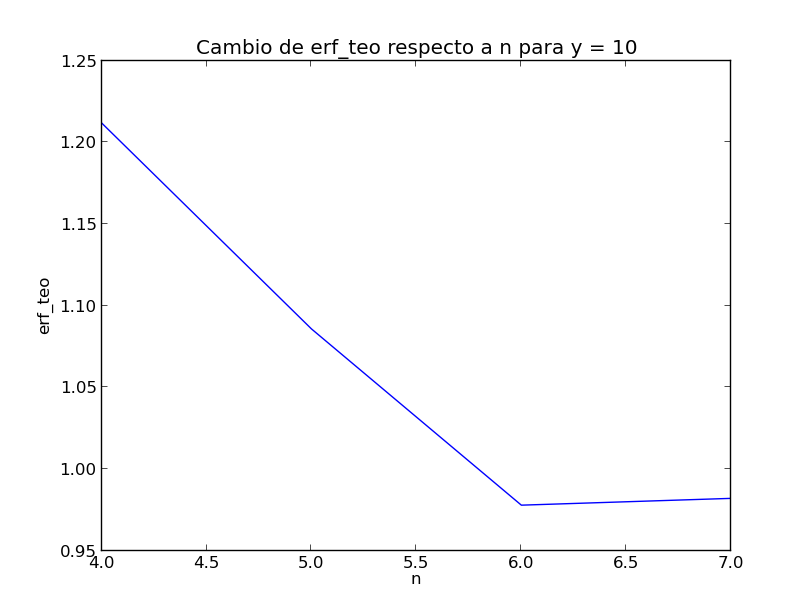
\includegraphics[width=400px]{preg4.png}

\subsubsection{Generación de erf\_real()}
Se nos pide desarrollar nuevamente una función que calcule la Función de Error de Gauss, pero que esta vez obtenga el valor real de la integración de la función.

El código fuente se puede analizar aquí:
\begin{verbatimtab}[4]
def erf_real(y):
	func = lambda x: e**(-x**2)
	return (2/(pi**(0.5)))*quad(func,0,y)[0]
\end{verbatimtab}

\subsubsection{Cálculo del Error Relativo}
Se nos pide calcular el error relativo para $y=10$, esto es:
\begin{center}
$\frac{|erf_t(y,n) - erf_r(y,n)|}{erf_r(y)}$
\end{center}

Lo cual entrega como resultado:
\begin{table}[!h]
\begin{center}
\begin{tabular}{|c|c|c|c|}
\hline
\textbf{$n$} & \textbf{erf\_teo} & \textbf{erf\_real} & \textbf{Error Relativo} \\ 
\hline \hline
$4$ & $1.2119475604$ & $1.0$ & $0.211947560402$ \\ \hline

$5$ & $1.08582368212$ & $1.0$ & $0.0858236821154$ \\ \hline

$6$ & $0.97790965366$ & $1.0$ & $0.0220903463402$ \\ \hline

$7$ & $0.982074829295$ & $1.0$ & $0.0179251707053$ \\ \hline
	\end{tabular}
\end{center}
\end{table}

\section{Conclusiones}
Podemos concluir que mediante métodos algorítmicos y gracias a la computación moderna, podemos simplificar el cálculo de data compleja, mediante métodos numéricos como las cuadraturas de Gauss, las cuales permiten obtener buenas estimaciones de los resultados reales. Esto es preciadamente útil para la computación ya que la máquina no es inteligente y es de recursos limitados.

Además, métodos como la interpolación polinomial responden adecuadamente a situcaciones donde la data puede ser difusa, y con funciones de naturaleza desconocida, las cuales se simplifican mediante métodos como splines o diferencias divididas, las cuales resultan ser aproximaciones a las curvas reales.
\end{document} 